%%%%%%%%%%%%%%%%%%%%%%%%%%%%%%%%%%%%%%%%%%%%%%%%%%%%%%%%%%%%%%%%%%%%%%%%

%%% LaTeX Template for ECAI Papers 
%%% Prepared by Ulle Endriss (version 1.0 of 2023-12-10)

%%% To be used with the ECAI class file ecai.cls.
%%% You also will need a bibliography file (such as mybibfile.bib).

%%%%%%%%%%%%%%%%%%%%%%%%%%%%%%%%%%%%%%%%%%%%%%%%%%%%%%%%%%%%%%%%%%%%%%%%

%%% Start your document with the \documentclass{} command.
%%% Use the first variant for the camera-ready paper.
%%% Use the second variant for submission (for double-blind reviewing).

%\documentclass{ecai} 
\documentclass[doubleblind]{ecai} 

%%%%%%%%%%%%%%%%%%%%%%%%%%%%%%%%%%%%%%%%%%%%%%%%%%%%%%%%%%%%%%%%%%%%%%%%

%%% Load any packages you require here. 

\usepackage{latexsym}
\usepackage{amssymb}
\usepackage{amsmath}
\usepackage{amsthm}
\usepackage{booktabs}
\usepackage{enumitem}
\usepackage{graphicx}
\usepackage{color}
\usepackage{hyperref}

%%%%%%%%%%%%%%%%%%%%%%%%%%%%%%%%%%%%%%%%%%%%%%%%%%%%%%%%%%%%%%%%%%%%%%%%

%%% Define any theorem-like environments you require here.

\newtheorem{theorem}{Theorem}
\newtheorem{lemma}[theorem]{Lemma}
\newtheorem{corollary}[theorem]{Corollary}
\newtheorem{proposition}[theorem]{Proposition}
\newtheorem{fact}[theorem]{Fact}
\newtheorem{definition}{Definition}

%%%%%%%%%%%%%%%%%%%%%%%%%%%%%%%%%%%%%%%%%%%%%%%%%%%%%%%%%%%%%%%%%%%%%%%%

%%% Define any new commands you require here.

\newcommand{\BibTeX}{B\kern-.05em{\sc i\kern-.025em b}\kern-.08em\TeX}

%%%%%%%%%%%%%%%%%%%%%%%%%%%%%%%%%%%%%%%%%%%%%%%%%%%%%%%%%%%%%%%%%%%%%%%%

\begin{document}

%%%%%%%%%%%%%%%%%%%%%%%%%%%%%%%%%%%%%%%%%%%%%%%%%%%%%%%%%%%%%%%%%%%%%%%%

\begin{frontmatter}

%%% Use this command to specify your submission number.
%%% In doubleblind mode, it will be printed on the first page.

\paperid{363} 

%%% Use this command to specify the title of your paper.

\title{Benchmarking Large Language Models for Bio-Image Analysis Code Generation}

%%% Use this combinations of commands to specify all authors of your 
%%% paper. Use \fnms{} and \snm{} to indicate everyone's first names 
%%% and surname. This will help the publisher with indexing the 
%%% proceedings. Please use a reasonable approximation in case your 
%%% name does not neatly split into "first names" and "surname".
%%% Specifying your ORCID digital identifier is optional. 
%%% Use the \thanks{} command to indicate one or more corresponding 
%%% authors and their email address(es). If so desired, you can specify
%%% author contributions using the \footnote{} command.

\author[A]{\fnms{First}~\snm{Author}\orcid{....-....-....-....}\thanks{Corresponding Author. Email: somename@university.edu.}\footnote{Equal contribution.}}
\author[B]{\fnms{Second}~\snm{Author}\orcid{....-....-....-....}\footnotemark}
\author[B,C]{\fnms{Third}~\snm{Author}\orcid{....-....-....-....}} 

\address[A]{Short Affiliation of First Author}
\address[B]{Short Affiliation of Second Author and Third Author}
\address[C]{Short Alternate Affiliation of Third Author}

%%% Use this environment to include an abstract of your paper.

\begin{abstract}
In the computational age we life in, life-scientists often solve scientific bio-image analysis (BIA) questions using Python code, even though they are not commonly trained in programming. As a common use-case for Large Language Models (LLMs) is code-generation, we see potential in using LLMs for BIA. We present a quantitative benchmark to estimate the capability of LLMs to generate code for solving common BIA tasks. The benchmark consists of 47 human-written prompts, corresponding canonical solutions written in Python and unit-tests to evaluate functional correctness of potential solutions. We demonstrate the benchmark by comparing 6 LLMs. We propose mid-/long-term efforts in maintaining and extending the benchmark by the BIA open-source community to ensure community needs are covered properly. This way we can also guide LLM developers in moving the frontier of current capabilities of LLMs towards more advanced applications in BIA. Our code is available on github.
\end{abstract}

\end{frontmatter}

%%%%%%%%%%%%%%%%%%%%%%%%%%%%%%%%%%%%%%%%%%%%%%%%%%%%%%%%%%%%%%%%%%%%%%%%

\section{Introduction}

Many projects in biology involve state-of-the-art microscopy and  quantitative bio-image analysis (BIA), which often requires programming skills. As programming is commonly not taught to life-scientists, we see a potential in using large language models for this task. Since modern Large Language Models (LLMs) such as chatGPT (OpenAI et al. 2023) were introduced, they change how humans interact with computers. LLMs were originally developed to solve  natural language processing tasks such as  text classification, language translation, or question answering. Interestingly, these models  are also capable of translating human languages, such as English, into programming languages, such as Python. Moreover, they can produce executable code that solves tasks defined by human natural language input (Brown et al. 2020). This capability has huge potential for interdisciplinary research areas such as microscopy image analysis (Loïc A. Royer 2023). LLMs can fill a gap where scientists with limited programming skills meet image analysis tasks which often require knowledge of programming languages such as Python. LLMs are indeed capable of writing BIA code as demonstrated in (Loic A. Royer 2023), but it is yet unclear where the limitations of this technology are in the BIA context. Thus, we think the bioimaging community urgently needs an openly accessible, quantitative way to measure those capabilities in particular given that LLM technology is also developing rapidly. We present such a benchmark, based on HumanEval (Chen et al. 2021), an established code-generation benchmark but ours is tailored for scientific questions in the Bio-Image Analysis context.

\begin{blind}
   \url{https://github.com/haesleinhuepf/human-eval-bia}
\end{blind}

%%%%%%%%%%%%%%%%%%%%%%%%%%%%%%%%%%%%%%%%%%%%%%%%%%%%%%%%%%%%%%%%%%%%%%%%

\section{Methods}

Our proposed benchmark consists of 47 human-written Python functions which contain documentation about what the function is supposed to do. An example is shown in Figure 1. This short documentation, the docstring, together with the function signature is passed to an LLM as part of a prompt asking to complete the code. The human-written implementation function body is not passed to the LLM, and just serves as a reference  solution. Additionally, our benchmark provides unit-tests for these python functions to evaluate their functional correctness. If the code generated by  the language model is executable and produces results which pass the unit-tests, this LLM is considered to be able to solve the problem described in the documentation of our function. Every prompt is sent multiple times to the LLM and we measure how often the generated  code passes the tests. Here, we follow the established standard pass@k (Chen et al. 2021), which estimates the probability that, if asked k times, the LLM will at least once give the correct answer. We particularly focus on the practically most relevant special case pass@1 , i.e. we want to know how likely it is that the first generated solution works.  
Our selected prompts range from basic image analysis tasks, such as applying an edge-preserving denoising filter to an image, over intermediate tasks such as labeling objects in a binary image or counting them (Figure 1), to challenging workflows including image processing steps, descriptive statistics, tabular data wrangling and dimensionality reduction. There is also a positive-control test-case, called return-hello-world, which is intentionally kept very simple to test if a specific LLM model is  capable of solving a trivial base task at all. A list of all test-cases and corresponding docstrings is given in Supplementary List 1.
To enable future extension and reproducing our benchmark, we provide the necessary infrastructure to turn the list of test-case Jupyter Notebooks into a JSON file that has the same format as the evaluation framework of HumanEval. We also did minor modifications to this framework to be able to execute the benchmark.
We demonstrate the benchmark by comparing the capabilities of a range of state-of-the-art  LLMs (covering commercial and freely available or open source models): gpt-3.5-turbo-1106, gpt-4-1106-preview, codellama (Rozière et al. 2023), claude-3-opus-20240229 (Anthropic 2024), gemini-pro (Pichai 2023),  Mistral-7B-Instruct-v0.2 (Jiang et al. 2023). Code for benchmarking gemini-1.5-pro and gemini-ultra are available as well, but could not be executed due to rate limits. 
For benchmarking the models, we generated 10 code samples of the 47 test-cases of the 6 models. Benchmarking was done on a Windows 10 Laptop with an AMD Ryzen 9 6900 CPU, 32 GB of RAM and a NVidia RTX 3050 TI GPU with 4 GB of RAM. Codellama, the only locally executed model in our selection, was accessed via ollama version 0.1.29 (Ollama 2024). The gemini-pro model was accessed via the Google Vertex API (Google Inc. 2024), which did not support specifying a version. Thus, we document here that the benchmark was executed on April 6th and 7th 2024. The Mistral model was accessed via the blablador infrastructure at the Jülich Supercomputing Centre in Germany.
All test-cases, benchmarking code, generated samples and data analysis/visualization notebooks are available open-source in the github repository of the project. All respective software versions are documented  in the environment.yml file in the Github repository:
https://github.com/haesleinhuepf/human-eval-bia/ 

\begin{figure}[h]
\centering
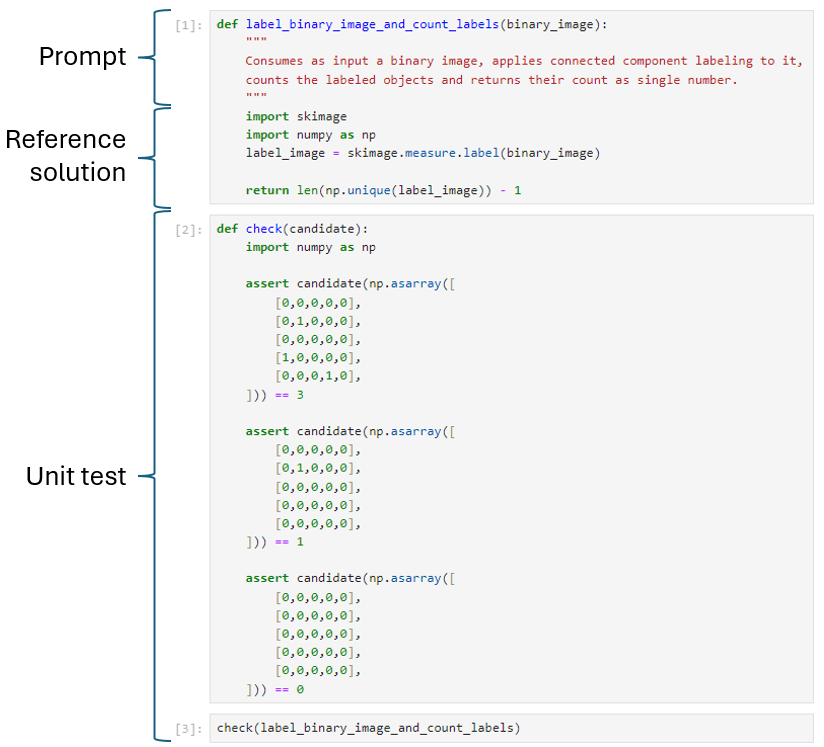
\includegraphics[width=8.5cm]{example_test_case.png}
\caption{Explanation comes here.}
\label{fig:exampletestcase}
\end{figure}


%%%%%%%%%%%%%%%%%%%%%%%%%%%%%%%%%%%%%%%%%%%%%%%%%%%%%%%%%%%%%%%%%%%%%%%%

\section{Results}

Execution of the sampling notebook took approximately 18 hours. The models gpt-3.5-turbo-1106, gpt4-1106-preview and claude-3-opus-20240229 caused costs of 0.23, 5.10 and 20.49, respectively. All other models did not cause direct costs as their API usage was free. Comparing the pass@k measurements reveals that the leading model, gpt-4-1106-preview, managed to answer 42 of the prompts with code that passed the unit tests. It is followed by claude-4-opus-20240229 and gpt-3.5-turbo-1106, with 40 and 28, respectively. These numbers correspond to pass1 counting the success rate from drawn examples. Detailed pass@k rates with k=1, k=5 and k=10 are shown in Figure 2 and Supplementary Table 1. 
Detailed analysis of the test-cases, shown in Table 1, highlights that most of the test-cases were solvable by at least one LLM. The positive control, return-hello-world, was solved successfully in almost all cases, expressed with a pass-rate of 100. Only the codellama model failed in 30 of the test runs for this particular test-case. Most advanced test-cases requiring implementation of advanced workflows were not solved by any of the LLMs.  

\begin{figure}[h]
\centering
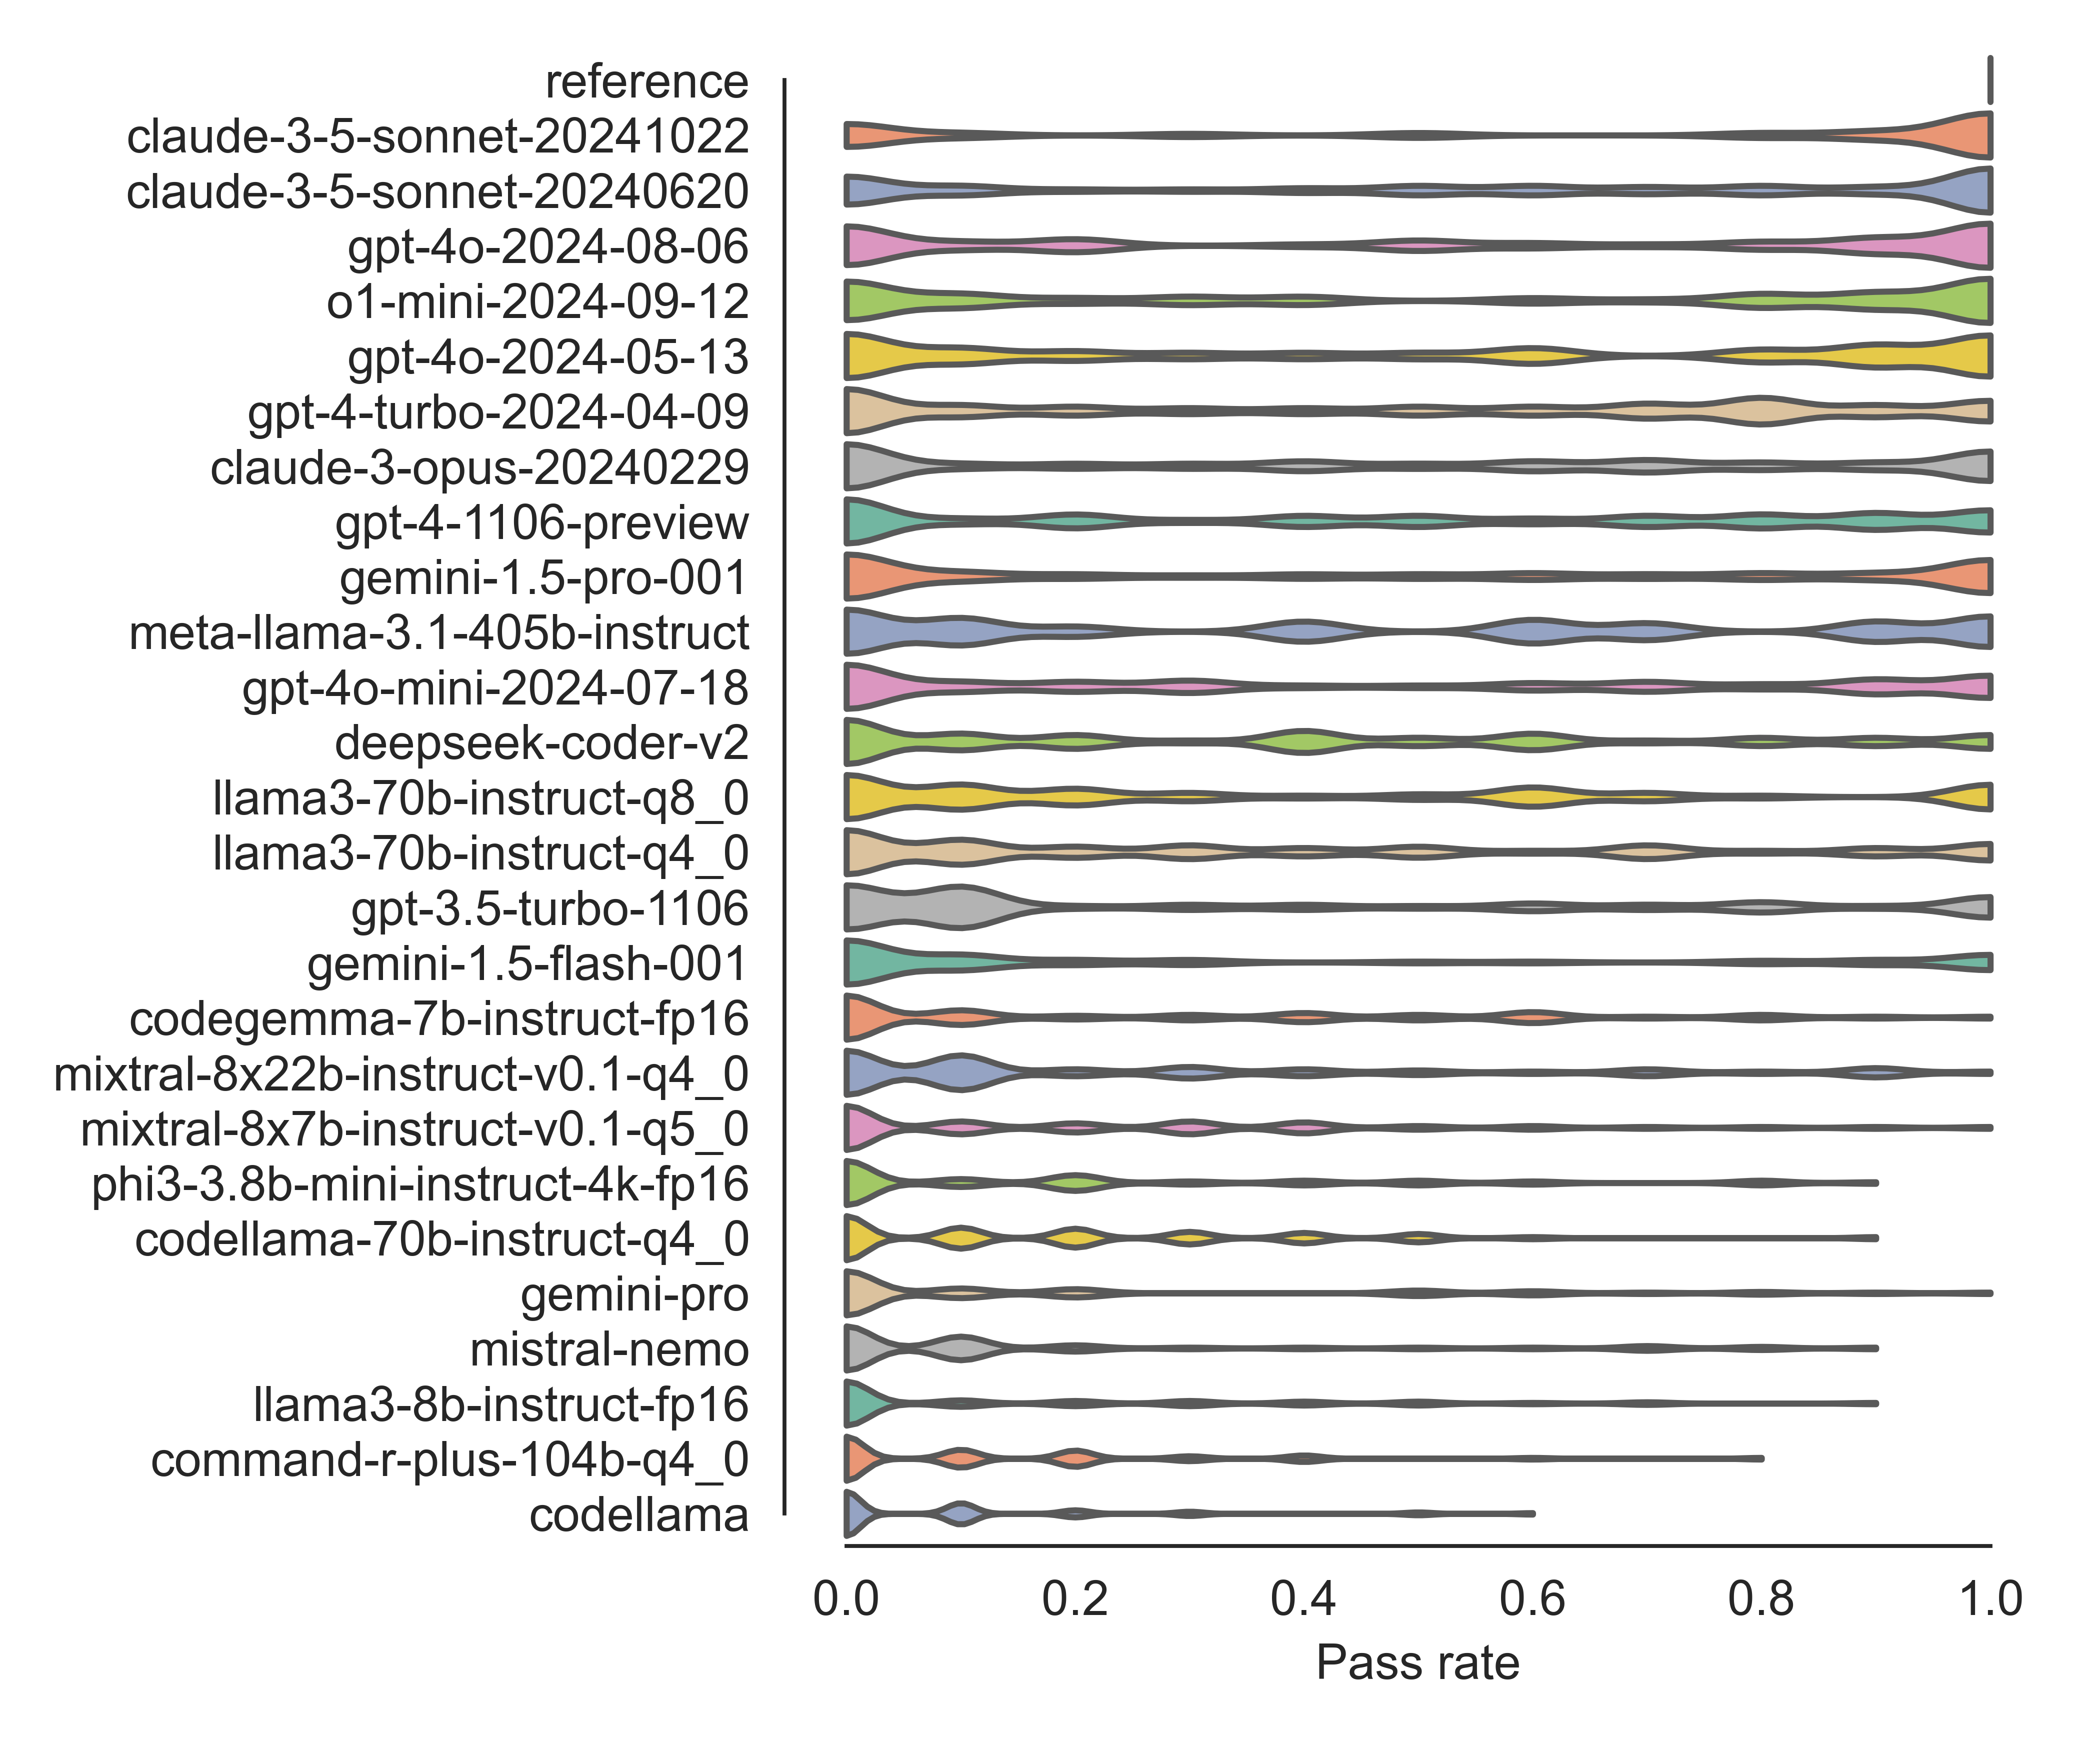
\includegraphics[width=8.5cm]{pass_rate_llms.png}
\caption{Explanation comes here.}
\label{fig:passratellms}
\end{figure}

\begin{figure*}[h]
\centering
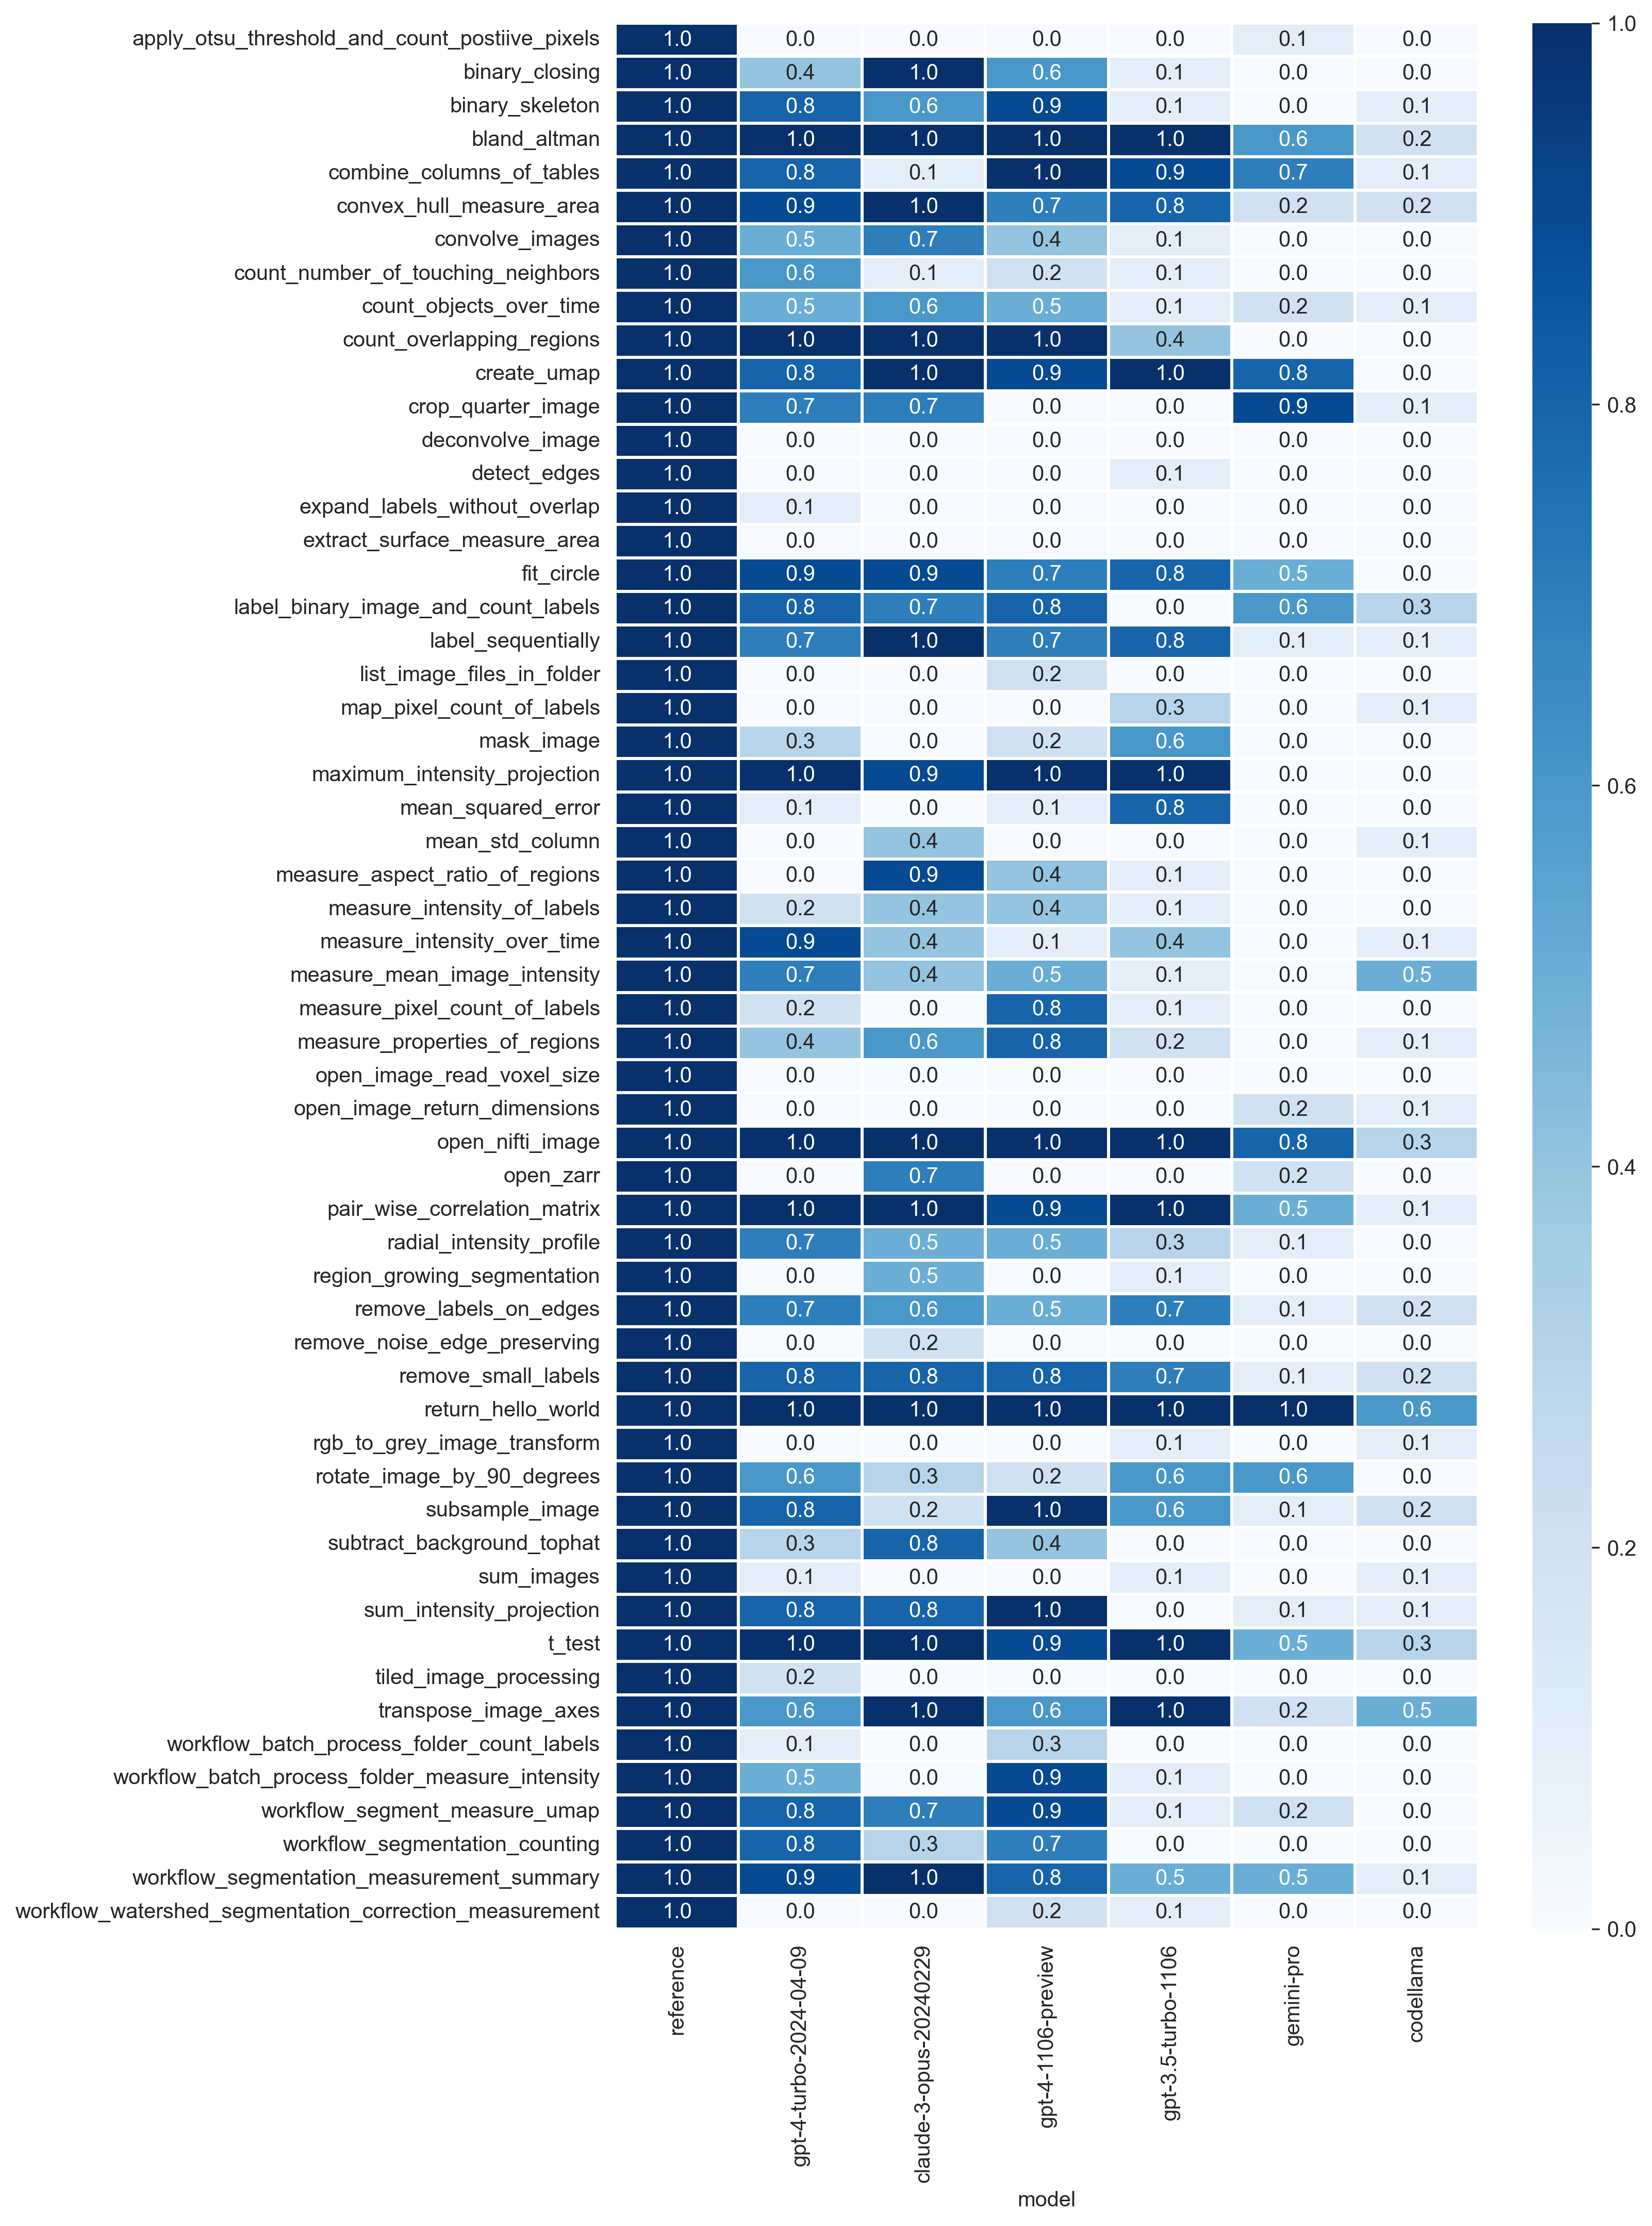
\includegraphics[width=\textwidth]{performance_per_task.png}
\caption{Explanation comes here.}
\label{fig:performancepertask}
\end{figure*}


%%%%%%%%%%%%%%%%%%%%%%%%%%%%%%%%%%%%%%%%%%%%%%%%%%%%%%%%%%%%%%%%%%%%%%%%

\section{Discussion}

We presented a benchmark for comparing code generation capabilities of LLMs in the Bio-image Analysis context. Such benchmarks are crucial to decide , e.g. if and how to apply this technology in routine projects, training or advanced applications. 
It shall be mentioned that we did not use any code-completion tools, such as github co-pilot, to write the test-cases. It is necessary to not use such LLM-based tools while writing the test-cases, because otherwise we might introduce a bias towards underlying LLMs. For example, github-copilot is based on chatGPT. If the test-cases were written using it, the benchmark might misleadingly reveal better performance of chatGPT.
Inspecting the detailed reports for which test-cases were not solved by any LLM also revealed a couple of cases, which are considered simple, but still were not solvable. Examples are list-files-in-folder, open-image-return-dimensions and rgb-to-grey-transform. Modifying such test-cases now, after a first benchmark has been executed, must be done carefully. A peer-review scheme, e.g. using github pull-requests, is recommended to make sure good scientific practice is maintained. Additionally, tools are available to the benchmark maintainers to detect if the LLMs are attempting to use Python libraries which are not installed yet. These can be added and the evaluation step repeated. As the maintainers only consider common Python libraries, the manual effort for this quality assurance step is limited. When maintaining this benchmark mid-/long-term modifications should only be done neutrally, to not give advantages to specific LLMs.
We limited sample generation for the benchmarking to 10 samples per LLM per test-case. pass@k analysis was done using k=1, k=5 and k=10. The established standard set by (Chen et al. 2021) is 200 samples and k=1, k=10 and k=100. As our benchmark is in early development (you are reading a preprint), we considered drawing 200 samples as not well-invested compute time and unnecessary costs. Once the benchmark contains more test-cases and models, this decision may be revised. 
The measured costs also demonstrate the potential of the technology. Requested code is commonly served within seconds, and drawing 300 samples from the 3 paid-per-prompt models causes minimal costs depending on the used model. When using LLMs on a daily basis, it appears unreasonable to draw hundreds of samples. Hence, using LLMs for BIA code generation is affordable and cost-efficient. 
Our benchmark is also a single-shot benchmark presenting the prompt to the LLM with no history of a former conversation. In daily use, one can interact with LLMs using chat-interfaces and iteratively engineer a prompt. Thus, the tested LLMs may be objectively more capable than measured in our experiment, when used in a chat scenario.
The test-case selection may introduce a certain bias of the sub-discipline we work in. We mostly work with fluorescence microscopy imaging data, showing nuclei and membranes. Most test-cases are derived from practical situations we come across often. Mid-/long-term we hope that community contributions to the benchmark’s github repository will allow us to reflect the field more broadly. For example, algorithms processing histological, hyperspectral, or super-resolution imaging data, would be welcome in our test-case collection. On the other hand, we consider test-cases without practical relevance in bio-image analysis should not be part of the benchmark. For example, an algorithm implementing image-reconstruction techniques for computed tomography, or image-classification algorithms for natural images, showing cats and dogs, should not be included even though they might fit technically in an image-processing benchmark. Also intentionally, we included test-case and prompts which we presume are currently not solvable by any LLM. With this, the benchmark could serve to guide LLM developers in this field.
We aim at developing this benchmark further, together with the support by the bio-image analysis community, by adding more test-cases. Furthermore, with the development of the models, we also will adapt the benchmark depending on how LLMs develop. For example, currently upcoming vision-models, LLMs that can take images as input, need to be considered for benchmarking too. The benchmark we presented does not have the capability to test vision-models. Another angle of further development could be efficiency of generated code as proposed earlier (Du et al. 2024). In particular in the context of processing 3D+t fluorescence microscopy imaging data, accelerated image processing techniques can by key (Haase et al. 2020). The presented benchmark could also be used to improve system messages systematically, for example in projects such as napari-chatGPT (Loic A. Royer 2023) and bia-bob projects (Haase, Tischer, and Yamauchi 2024).

%%%%%%%%%%%%%%%%%%%%%%%%%%%%%%%%%%%%%%%%%%%%%%%%%%%%%%%%%%%%%%%%%%%%%%%%

\section{Conclusion}

We developed a benchmark for measuring LLM performance in generating code for solving BIA task. It can guide end-users to decide which LLM to use and potentially to pay for when using them for bio-image analysis coding tasks. We also consider this benchmark for LLM-developers in our domain as a metric to guide further development. Last but not least: We encourage the community to send pull-requests with new test-cases to the above-mentioned github repository to ensure the benchmark is covering needs in our field widely. This way, we wish to establish a community-driven approach to benchmarking LLMs for BIA. 



%%%%%%%%%%%%%%%%%%%%%%%%%%%%%%%%%%%%%%%%%%%%%%%%%%%%%%%%%%%%%%%%%%%%%%%%


\section{Citations and references}

Include full bibliographic information for everything you cite, 
be it a book \citep{pearl2009causality}, a journal article 
\citep{grosz1996collaborative,rumelhart1986learning,turing1950computing}, 
a conference paper \citep{kautz1992planning}, or a preprint 
\citep{perelman2002entropy}. The citations in the previous sentence are 
known as \emph{parenthetical} citations, while this reference to the 
work of \citet{turing1950computing} is an \emph{in-text} citation.
The use of \BibTeX\ is highly recommended. 

%%%%%%%%%%%%%%%%%%%%%%%%%%%%%%%%%%%%%%%%%%%%%%%%%%%%%%%%%%%%%%%%%%%%%%%%

%%% Use this environment to include acknowledgements (optional).
%%% This will be omitted in doubleblind mode.

\begin{ack}
RH acknowledges the financial support by the Federal Ministry of Education and Research of Germany and by Sächsische Staatsministerium für Wissenschaft, Kultur und Tourismus in the programme Center of Excellence for AI-research „Center for Scalable Data Analytics and Artificial Intelligence Dresden/Leipzig“, project identification number: ScaDS.AI.
Helmholtz AI and the Jülich Supercomputing Centre deserve acknowledgement for providing the blablador infrastructure for testing the mistral model.
\end{ack}

%%%%%%%%%%%%%%%%%%%%%%%%%%%%%%%%%%%%%%%%%%%%%%%%%%%%%%%%%%%%%%%%%%%%%%%%

%%% Use this command to include your bibliography file.

\bibliography{mybibfile}

\end{document}
%%%%%%%%%%%%%%%%%%%%%%%%%%%%%%%%%%%%%%%%%%%%%%%%%%%%%%%%%%%%%%%%%%%%%%
